\section{Implementation Details}
\label{app:impl}

\paragraph{Renderer.}
Pages are 1008 pixels wide (36 patches) with a 4-pixel margin and are rendered in grayscale with the Menlo monospace font through PIL.
Prose is wrapped at character boundaries; a flagged word is placed whole on the next line when it does not fit.
Each line is as tall as its largest glyph plus one pixel of leading.
Documents taller than 2016 pixels are split into pages at blank pixel rows, so no line is cut; all pages are sent in one request in reading order.
The budget of \cref{eq:vtok} is enforced on the unsplit image; splitting can add one patch row per page, which made 10 of the 180 reallocated long-context images 1.2\% more expensive than their uniform counterparts.
All reported costs are billed tokens and include this effect.

\paragraph{Detector.}
After stripping the characters \texttt{.,;:()[]"'} from both ends, a word is flagged if it matches \verb![0-9a-f]{8,}!, \verb!\d{5,}!, \verb!/\S*\d\S*!, \verb!\d+\.\d+\.\d+\.\d+!, \verb!\S+/\S+\.\w{1,5}!, or \verb!sha256=!, or if it contains at least one letter and one digit and either contains \verb![A-Za-z0-9_\-]{20,}! or is at least 16 characters long with a 16-character window whose character entropy is at least 3.5 bits.

\paragraph{Baselines.}
U tries Menlo, Arial, and Arial Narrow at sizes 14 down to 5\,px and keeps the largest size that fits the budget (ties broken by font order); at the 5\,px and 6\,px budgets it selects 6\,px Arial and 8\,px Arial Narrow for most documents.
Z renders at 10\,px and shrinks the image by repeated factors of 0.98 with Lanczos resampling until it fits the budget (final scale 0.52--0.64).
For RULER and the natural-identifier questions, K and X append, after the question, the line ``Exact strings copied verbatim from the text block in the image:'' followed by one flagged string per line; for LongBench, the anchors are inserted after the image placeholder and before the question, under ``Exact strings copied verbatim from the text in the image:''.

\paragraph{Prompts and scoring.}
RULER prompts follow the official template with the context replaced by ``[The text is rendered in the image above.]'', add ``Copy each one exactly, character for character.'', and ask for a JSON list of values; a gold value counts as recalled if it appears (case-insensitively) in any returned string.
LongBench prompts are the official ones for each task; the first output line is scored with the official QA F1.
For the plain-text arm the context is inserted verbatim into the same template.

\paragraph{Router threshold.}
$\tau$ is chosen per reader by two-fold cross-validation on the density sweep (folds by item parity), maximizing recall minus 0.5 times the cost relative to plain text over $\tau\in\{0,0.05,0.1,0.2,0.3,0.5,0.75,1,1.5,2,4,\infty\}$.
Selected values were 0.1--0.5 with median 0.3, which we use for all other experiments. The frontier in \cref{fig:density}c sweeps $\tau$ and the per-density figures use the median $\tau$; both are therefore in-sample, unlike the cross-validated aggregate.

\section{Per-Reader Results}
\label{app:tables}

\Cref{tab:app_length,tab:app_density} give per-reader numbers for \cref{fig:scaling,fig:density}.

\begin{table}[!htbp]
\centering\small\setlength{\tabcolsep}{4pt}
\caption{Per-reader recall for the length study (\cref{fig:scaling}). The mean excludes Claude.}
\label{tab:app_length}
\begin{tabular}{l cc cc cc}
\toprule
& \multicolumn{2}{c}{32K} & \multicolumn{2}{c}{64K} & \multicolumn{2}{c}{128K} \\
\cmidrule(lr){2-3}\cmidrule(lr){4-5}\cmidrule(lr){6-7}
Reader & A & S & A & S & A & S \\
\midrule
Claude Sonnet 5.5 & 0.57 & \textbf{0.86} & 0.51 & \textbf{0.96} & 0.45 & \textbf{0.97} \\
Gemini 3.5 Flash-Lite & 0.47 & \textbf{0.91} & 0.26 & \textbf{0.74} & 0.21 & \textbf{0.70} \\
GPT-6 Luna & 0.09 & \textbf{0.59} & 0.12 & \textbf{0.55} & 0.09 & \textbf{0.50} \\
Qwen3-VL-235B & 0.02 & \textbf{0.60} & 0.02 & \textbf{0.55} & 0.06 & \textbf{0.54} \\
Llama 4 Maverick & 0.01 & \textbf{0.50} & 0.00 & \textbf{0.54} & 0.00 & \textbf{0.47} \\
MiniMax-M3 & 0.00 & \textbf{0.40} & 0.00 & \textbf{0.49} & 0.00 & \textbf{0.56} \\
\midrule
\textit{Mean} & 0.12 & 0.60 & 0.08 & 0.57 & 0.07 & 0.56 \\
\bottomrule
\end{tabular}
\end{table}

\begin{table}[t]
\centering
\caption{\textbf{Detector ablation.} RULER multi-value recall (16K characters, 6\,px budget, $N{=}25$, mean of 5 readers; Claude was not run in this ablation). Seven-digit values are flagged by the regex detector; four-digit values are deliberately not (they collide with years), so the regex arms fall back to uniform rendering.}
\label{tab:detector}
\small
\setlength{\tabcolsep}{5pt}
\begin{tabular}{l cc}
\toprule
& 7-digit values & 4-digit values \\
Arm & (detected) & (missed) \\
\midrule
Uniform (A) & 0.22 & 0.32 \\
\midrule
Ours, regex detector (S) & 0.77 & 0.33 \\
Ours, oracle detector & 0.78 & 0.82 \\
Ours + anchors, regex (X) & 0.99 & 0.32 \\
Ours + anchors, oracle & 0.99 & 0.99 \\
\bottomrule
\end{tabular}
\end{table}


\section{Statistical Procedures}
\label{app:stats}

\paragraph{Metrics.}
Recall is the fraction of gold values that appear, case-insensitively, as a substring of some returned value.
The precision-aware F1 deduplicates the returned values, counts a returned value as correct when it contains a gold value, and combines this precision with recall; an empty answer scores zero.
Exact-set accuracy requires every gold value to be found and no other value to be returned.
Outputs that cannot be parsed are scored as empty answers; empty responses and transport errors are dropped (\cref{sec:setup}).

\paragraph{Per-cell tests.}
For one reader on one task at one setting, we bootstrap the mean paired difference over items (10{,}000 resamples for the per-cell intervals reported in tables, 1{,}000 for the $p$-values used for Holm correction) and call the cell significant when the two-sided bootstrap $p$-value is below 0.05.

\paragraph{Pooled effects.}
The pooled effect is the mean paired difference over all (run, reader, item) triples of a family, where a family is one row of \cref{tab:pooled}.
The item-level interval resamples items within each run, with the same item draw for every reader, so it treats the five readers as fixed.
The reader-and-item interval additionally resamples readers with replacement; one reader draw is shared by all runs of the family because readers are crossed with runs.
Both use 4{,}000 resamples and percentile intervals.
Within each family we apply Holm's step-down correction to the per-cell $p$-values and report how many cells remain significant in each direction.
\Cref{tab:app_pooled} lists every comparison we computed, including those not discussed in the main text.

\begin{table}[!htbp]
\centering
\caption{\textbf{All pooled comparisons, RULER at 16K characters} (five non-Claude readers; recall and precision-aware F1). CI$_{\mathrm{item}}$ resamples items within each run with the readers fixed. CI$_{\mathrm{rd+item}}$ also resamples readers (one draw shared by all runs). Cells are counted as significantly positive/negative by per-cell bootstrap, raw and after Holm correction within the row.}
\label{tab:app_pooled}
\footnotesize
\setlength{\tabcolsep}{3pt}
\begin{tabular}{l l l r c c c c r}
\toprule
Setting & Comparison & Metric & $\Delta$ & CI$_{\mathrm{item}}$ & CI$_{\mathrm{rd+item}}$ & raw $+/-$ & Holm $+/-$ & cells \\
\midrule
RULER 16K, 5\,px & S$-$A & recall & +0.55 & [+0.50, +0.60] & [+0.48, +0.62] & 14/0 & 14/0 & 15 \\
 &  & F1 & +0.46 & [+0.41, +0.50] & [+0.39, +0.54] & 14/0 & 14/0 & 15 \\
RULER 16K, 5\,px & S$-$U & recall & +0.52 & [+0.47, +0.56] & [+0.44, +0.60] & 14/0 & 13/0 & 15 \\
 &  & F1 & +0.42 & [+0.38, +0.46] & [+0.37, +0.47] & 13/0 & 13/0 & 15 \\
RULER 16K, 5\,px & S$-$Z & recall & +0.47 & [+0.43, +0.52] & [+0.34, +0.59] & 13/0 & 13/0 & 15 \\
 &  & F1 & +0.38 & [+0.34, +0.42] & [+0.29, +0.46] & 13/0 & 13/0 & 15 \\
RULER 16K, 5\,px & S$-$R & recall & +0.54 & [+0.49, +0.58] & [+0.47, +0.60] & 14/0 & 14/0 & 15 \\
 &  & F1 & +0.45 & [+0.41, +0.48] & [+0.39, +0.50] & 14/0 & 14/0 & 15 \\
RULER 16K, 5\,px & X$-$K & recall & +0.01 & [-0.01, +0.02] & [-0.02, +0.04] & 0/0 & 0/0 & 15 \\
 &  & F1 & 0.00 & [-0.01, +0.02] & [-0.02, +0.03] & 0/0 & 0/0 & 15 \\
RULER 16K, 6\,px & S$-$A & recall & +0.43 & [+0.39, +0.47] & [+0.27, +0.56] & 11/0 & 11/0 & 15 \\
 &  & F1 & +0.34 & [+0.30, +0.37] & [+0.21, +0.45] & 11/0 & 9/0 & 15 \\
RULER 16K, 6\,px & S$-$U & recall & +0.44 & [+0.40, +0.48] & [+0.31, +0.55] & 11/0 & 11/0 & 15 \\
 &  & F1 & +0.35 & [+0.31, +0.38] & [+0.26, +0.43] & 11/0 & 10/0 & 15 \\
RULER 16K, 6\,px & S$-$Z & recall & +0.47 & [+0.42, +0.51] & [+0.30, +0.60] & 11/0 & 11/0 & 15 \\
 &  & F1 & +0.38 & [+0.34, +0.41] & [+0.24, +0.49] & 11/0 & 11/0 & 15 \\
RULER 16K, 6\,px & S$-$R & recall & +0.56 & [+0.51, +0.60] & [+0.47, +0.64] & 12/0 & 12/0 & 15 \\
 &  & F1 & +0.47 & [+0.43, +0.50] & [+0.38, +0.55] & 12/0 & 12/0 & 15 \\
RULER 16K, 6\,px & X$-$K & recall & +0.05 & [+0.03, +0.08] & [0.00, +0.12] & 3/0 & 1/0 & 15 \\
 &  & F1 & +0.04 & [+0.01, +0.06] & [0.00, +0.08] & 2/0 & 1/0 & 15 \\
RULER 16K, 6\,px (box runs) & B$-$A & recall & -0.05 & [-0.07, -0.03] & [-0.13, 0.00] & 0/3 & 0/1 & 15 \\
 &  & F1 & -0.05 & [-0.07, -0.03] & [-0.13, 0.00] & 0/3 & 0/1 & 15 \\
RULER 16K, 6\,px (box runs) & S$-$B & recall & +0.53 & [+0.50, +0.57] & [+0.41, +0.64] & 14/0 & 14/0 & 15 \\
 &  & F1 & +0.45 & [+0.42, +0.49] & [+0.36, +0.56] & 14/0 & 14/0 & 15 \\
RULER 16K, 6\,px (box runs) & S$-$A & recall & +0.49 & [+0.45, +0.52] & [+0.29, +0.63] & 13/0 & 13/0 & 15 \\
 &  & F1 & +0.40 & [+0.37, +0.44] & [+0.26, +0.53] & 14/0 & 14/0 & 15 \\
\bottomrule
\end{tabular}
\end{table}


\section{Precision-Aware Scoring and Anchor Content}
\label{app:rescore}

\Cref{tab:app_rescore} reports, for every RULER setting with anchors, recall and precision-aware F1 for A, S, K, and X, how many values each arm returns, and two baselines that never look at the image: returning every anchor (dump) and returning as many random anchors as there are gold values (pick).
Three observations qualify the anchor results in the main text.
First, on single and multi-value the anchors are exactly the needles, so K and X match the dump baseline and their recall says nothing about reading.
Second, on multi-key and in the density sweep at $k{\ge}4$, several readers (Qwen3-VL and MiniMax most often) return most or all of the anchor list; recall stays high while F1 falls to the level of the pick baseline.
Third, uniform rendering sometimes produces long lists of hallucinated identifiers (up to 55 per item for MiniMax at 5\,px), which F1 penalizes and recall does not; the gains of S over A are therefore smaller under F1 but remain significant (\cref{tab:app_pooled}).
On the natural-identifier questions, readers return one value per question for every arm, so recall and F1 coincide.

\begin{table*}[h]
\centering
\caption{\textbf{Precision-aware rescoring and anchor content} (means over five readers). rec: recall; F1: precision-aware F1 over the returned values; \#ret: values returned per item; \#anc: distinct anchors per item; dump: recall of returning every anchor; pick: expected recall of returning as many random anchors as there are gold values. Neither copy baseline looks at the image. On single and multi-value the anchor list contains exactly the needles, so K and X approach the dump baseline; at $k{\ge}4$ several readers return most of the list, which recall rewards and F1 does not.}
\label{tab:app_rescore}
\footnotesize
\setlength{\tabcolsep}{3pt}
\resizebox{\textwidth}{!}{%
\begin{tabular}{l ccc ccc ccc ccc ccc}
\toprule
& \multicolumn{3}{c}{A} & \multicolumn{3}{c}{S} & \multicolumn{3}{c}{K} & \multicolumn{3}{c}{X} & \multicolumn{3}{c}{anchor list} \\
\cmidrule(lr){2-4}\cmidrule(lr){5-7}\cmidrule(lr){8-10}\cmidrule(lr){11-13}\cmidrule(lr){14-16}
Setting & rec & F1 & \#ret & rec & F1 & \#ret & rec & F1 & \#ret & rec & F1 & \#ret & \#anc & dump & pick \\
\midrule
16K, 5\,px, single & 0.02 & 0.02 & 1.4 & 0.42 & 0.41 & 0.9 & 0.99 & 0.99 & 1.0 & 0.98 & 0.98 & 1.0 & 1.0 & 1.00 & 1.00 \\
16K, 5\,px, multi-key & 0.11 & 0.11 & 13.8 & 0.77 & 0.48 & 2.8 & 0.98 & 0.46 & 3.6 & 0.99 & 0.47 & 3.7 & 4.2 & 1.00 & 0.24 \\
16K, 5\,px, multi-value & 0.12 & 0.13 & 10.1 & 0.73 & 0.76 & 3.5 & 0.96 & 0.95 & 4.0 & 0.97 & 0.97 & 4.0 & 4.2 & 1.00 & 0.96 \\
16K, 6\,px, single & 0.16 & 0.16 & 1.1 & 0.40 & 0.40 & 1.1 & 0.98 & 0.98 & 1.0 & 1.00 & 1.00 & 1.0 & 1.0 & 1.00 & 0.98 \\
16K, 6\,px, multi-key & 0.24 & 0.24 & 4.5 & 0.77 & 0.48 & 2.8 & 0.94 & 0.49 & 3.2 & 1.00 & 0.52 & 3.5 & 4.2 & 1.00 & 0.24 \\
16K, 6\,px, multi-value & 0.25 & 0.28 & 3.5 & 0.79 & 0.81 & 3.6 & 0.90 & 0.91 & 3.7 & 0.99 & 0.97 & 4.1 & 4.3 & 1.00 & 0.96 \\
density $k{=}1$ & 0.04 & 0.04 & 1.1 & 0.42 & 0.42 & 0.9 & 0.98 & 0.97 & 1.0 & 1.00 & 0.97 & 1.1 & 1.5 & 1.00 & 0.83 \\
density $k{=}4$ & 0.03 & 0.03 & 1.1 & 0.40 & 0.25 & 2.9 & 0.93 & 0.48 & 3.2 & 0.98 & 0.42 & 3.8 & 4.0 & 1.00 & 0.25 \\
density $k{=}16$ & 0.02 & 0.02 & 1.7 & 0.24 & 0.17 & 5.1 & 0.70 & 0.25 & 8.3 & 0.80 & 0.27 & 9.8 & 16.4 & 1.00 & 0.06 \\
density $k{=}64$ & 0.03 & 0.03 & 2.8 & 0.06 & 0.06 & 5.6 & 0.34 & 0.16 & 10.0 & 0.32 & 0.13 & 10.8 & 64.2 & 1.00 & 0.02 \\
multi-key 64K & 0.11 & 0.11 & 4.8 & 0.79 & 0.39 & 3.3 & 0.94 & 0.38 & 4.2 & 0.99 & 0.40 & 4.3 & 4.8 & 1.00 & 0.22 \\
multi-key 128K & 0.11 & 0.10 & 16.6 & 0.75 & 0.38 & 3.3 & 0.96 & 0.39 & 4.7 & 0.97 & 0.36 & 5.1 & 6.0 & 1.00 & 0.18 \\
\bottomrule
\end{tabular}}
\end{table*}


\Cref{tab:app_silent} gives the rate of well-formed near-misses on RULER: a gold value counts as a near-miss when it was not recalled but some returned string has the same length and at least 60\% character similarity.
Allocation does not reduce this rate; it rises from 0.12 to 0.15 at 5\,px and from 0.08 to 0.15 at 6\,px on average, plausibly because allocation turns many complete misses into nearly correct readings, some of which are still wrong; anchors nearly remove near-misses where they contain the answer.
We therefore do not claim that allocation makes errors detectable; check-and-retry~\cite{anon2026renderretain} addresses that problem.

\begin{table}[h]
\centering
\caption{\textbf{Well-formed near-misses} on RULER (16K): fraction of gold values for which the reader returned a different string of the same length with at least 60\% character similarity. Allocation does not reduce this rate; anchors nearly remove it.}
\label{tab:app_silent}
\small
\setlength{\tabcolsep}{3pt}
\resizebox{\columnwidth}{!}{%
\begin{tabular}{l ccccc ccccc}
\toprule
& \multicolumn{5}{c}{5\,px budget} & \multicolumn{5}{c}{6\,px budget} \\
\cmidrule(lr){2-6}\cmidrule(lr){7-11}
Reader & A & U & Z & S & K & A & U & Z & S & K \\
\midrule
Gemini & 0.50 & 0.32 & 0.13 & 0.00 & 0.00 & 0.06 & 0.15 & 0.09 & 0.00 & 0.00 \\
GPT & 0.05 & 0.03 & 0.01 & 0.15 & 0.01 & 0.08 & 0.07 & 0.12 & 0.15 & 0.00 \\
Qwen & 0.01 & 0.02 & 0.01 & 0.25 & 0.00 & 0.14 & 0.12 & 0.14 & 0.14 & 0.00 \\
Llama & 0.02 & 0.02 & 0.01 & 0.25 & 0.00 & 0.05 & 0.17 & 0.10 & 0.21 & 0.02 \\
MiniMax & 0.00 & 0.00 & 0.00 & 0.13 & 0.00 & 0.07 & 0.07 & 0.08 & 0.23 & 0.00 \\
\midrule
\textit{Mean} & 0.12 & 0.08 & 0.03 & 0.15 & 0.00 & 0.08 & 0.11 & 0.10 & 0.15 & 0.00 \\
\bottomrule
\end{tabular}}
\end{table}


\section{Controls, Milder Budgets, and Replication}
\label{app:controls}

\Cref{tab:app_controls} gives per-reader results for the box control and the milder budgets of \cref{sec:main,sec:regime}, and \cref{fig:examples} shows one item from the box runs.
The box runs used a fresh sample of 25 items per task and re-read A and S, which serves as a replication of \cref{tab:baselines}: on the new items, A averages 0.20 and S 0.68, against 0.22 and 0.65 on the original items at the same budget.
At 8 and 10\,px the U arm switches to Arial Narrow at 10 and 13\,px, which is why it catches up with S at the lighter budget; anchors (K, X) reach 0.96--1.00 at both budgets because the anchors again contain the needles.

\begin{figure*}[h]
\centering
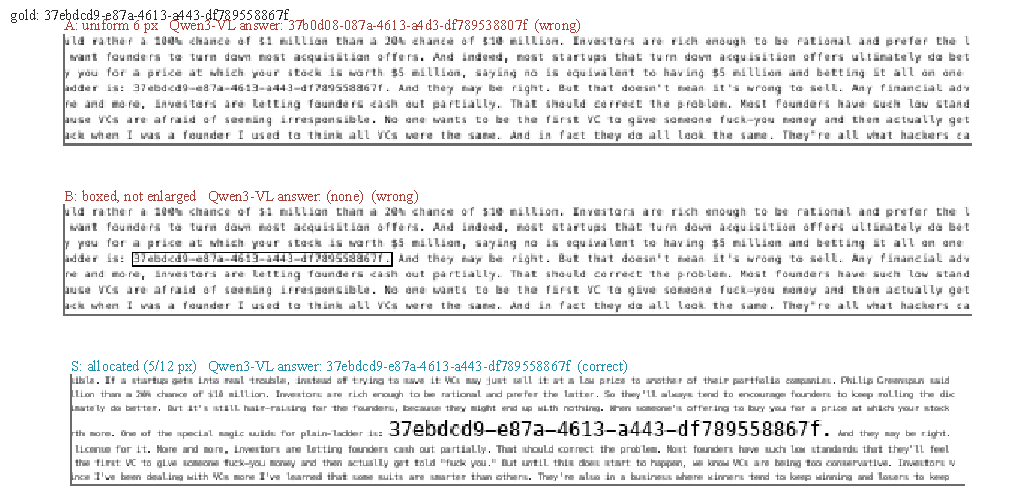
\includegraphics[width=\textwidth]{fig/examples.pdf}
\caption{\textbf{One RULER item at the 6\,px budget} (crops around the needle; Qwen3-VL answers). Uniform rendering yields a well-formed UUID with several wrong characters; boxing the needle at the same size does not help (the reader returned nothing); allocation draws the UUID at 12\,px and prose at 5\,px, and the answer is exact.}
\label{fig:examples}
\end{figure*}

\begin{table*}[h]
\centering
\caption{\textbf{Salience control and milder budgets} (recall per reader; box control averages three RULER tasks on a fresh sample of 25 items each, milder budgets average single and multi-key). B boxes the flagged strings without enlarging them.}
\label{tab:app_controls}
\small
\setlength{\tabcolsep}{3pt}
\resizebox{\textwidth}{!}{%
\begin{tabular}{l ccc ccccc ccccc}
\toprule
& \multicolumn{3}{c}{Box control, 16K, 6\,px} & \multicolumn{5}{c}{32K, 8\,px} & \multicolumn{5}{c}{32K, 10\,px} \\
\cmidrule(lr){2-4}\cmidrule(lr){5-9}\cmidrule(lr){10-14}
Reader & A & B & S & A & U & S & K & X & A & U & S & K & X \\
\midrule
Gemini & 0.87 & 0.67 & 1.00 & 0.48 & 0.42 & 0.90 & 0.96 & 1.00 & 0.68 & 0.84 & 0.92 & 0.98 & 1.00 \\
GPT & 0.09 & 0.07 & 0.77 & 0.14 & 0.34 & 0.54 & 1.00 & 0.98 & 0.50 & 0.68 & 0.74 & 0.90 & 1.00 \\
Qwen & 0.02 & 0.00 & 0.58 & 0.14 & 0.28 & 0.48 & 1.00 & 1.00 & 0.44 & 0.58 & 0.62 & 1.00 & 1.00 \\
Llama & 0.00 & 0.00 & 0.56 & 0.00 & 0.18 & 0.44 & 0.88 & 1.00 & 0.16 & 0.36 & 0.38 & 0.92 & 0.96 \\
MiniMax & 0.00 & 0.00 & 0.50 & 0.00 & 0.10 & 0.28 & 1.00 & 1.00 & 0.22 & 0.36 & 0.36 & 1.00 & 0.98 \\
\midrule
\textit{Mean} & 0.20 & 0.15 & 0.68 & 0.15 & 0.26 & 0.53 & 0.97 & 1.00 & 0.40 & 0.56 & 0.60 & 0.96 & 0.99 \\
\textit{Billed} & 929 & 923 & 843 & 1913 & 1855 & 1890 & 1954 & 1931 & 3061 & 2870 & 2826 & 3101 & 2866 \\
\bottomrule
\end{tabular}}
\end{table*}


\section{Anchors: Budget Frontier and Long Context}
\label{app:anchors}

\Cref{tab:app_niqfront} gives the per-reader numbers behind the frontier of \cref{sec:anchors}: the 60 flagged natural-identifier questions rendered at base sizes of 5, 6, and 7\,px.
Allocation alone gains 0.19--0.25 over uniform rendering at every budget, and anchors add 0.28--0.37 on top of S and 0.46--0.53 on top of A.
\Cref{tab:app_longkx} gives multi-key results at 64K and 128K characters: recall separates the arms, but F1 does not, because every arm with enlarged or copied values tends to return several candidates for the one queried key.

\begin{table*}[h]
\centering
\caption{\textbf{Natural identifiers at three budgets} (flagged targets, $N{=}60$, recall). Billed tokens average the four readers that report usage. X is at or above K at every budget and costs the same as K at 5\,px, where prose cannot shrink.}
\label{tab:app_niqfront}
\small
\setlength{\tabcolsep}{3pt}
\resizebox{\textwidth}{!}{%
\begin{tabular}{l cccc cccc cccc}
\toprule
& \multicolumn{4}{c}{5\,px} & \multicolumn{4}{c}{6\,px} & \multicolumn{4}{c}{7\,px} \\
\cmidrule(lr){2-5}\cmidrule(lr){6-9}\cmidrule(lr){10-13}
Reader & A & S & K & X & A & S & K & X & A & S & K & X \\
\midrule
Gemini & 0.62 & 0.75 & 0.92 & 0.90 & 0.72 & 0.80 & 0.87 & 0.90 & 0.77 & 0.85 & 0.92 & 0.85 \\
GPT & 0.17 & 0.47 & 0.80 & 0.83 & 0.25 & 0.55 & 0.85 & 0.82 & 0.35 & 0.55 & 0.87 & 0.88 \\
Qwen & 0.03 & 0.32 & 0.68 & 0.75 & 0.12 & 0.48 & 0.77 & 0.78 & 0.20 & 0.48 & 0.77 & 0.77 \\
Llama & 0.03 & 0.17 & 0.53 & 0.58 & 0.05 & 0.20 & 0.55 & 0.62 & 0.10 & 0.37 & 0.67 & 0.83 \\
MiniMax & 0.03 & 0.22 & 0.63 & 0.68 & 0.03 & 0.39 & 0.65 & 0.67 & 0.15 & 0.27 & 0.62 & 0.73 \\
\midrule
\textit{Mean} & 0.18 & 0.38 & 0.71 & 0.75 & 0.23 & 0.48 & 0.74 & 0.76 & 0.31 & 0.50 & 0.77 & 0.81 \\
\textit{Billed} & 936 & 940 & 1014 & 1017 & 1181 & 1035 & 1267 & 1128 & 1267 & 1218 & 1345 & 1306 \\
\bottomrule
\end{tabular}}
\end{table*}

\begin{table}[!htbp]
\centering
\caption{\textbf{Anchors at long context} (RULER multi-key, 6\,px, $N{=}20$; recall and precision-aware F1). Allocation makes X 29--31\% cheaper than K, but under F1 the three arms S, K, and X are indistinguishable.}
\label{tab:app_longkx}
\footnotesize
\setlength{\tabcolsep}{3pt}
\begin{tabular}{l cccccccccccccccc}
\toprule
& \multicolumn{8}{c}{64K characters} & \multicolumn{8}{c}{128K characters} \\
\cmidrule(lr){2-9}\cmidrule(lr){10-17}
& \multicolumn{2}{c}{A} & \multicolumn{2}{c}{S} & \multicolumn{2}{c}{K} & \multicolumn{2}{c}{X} & \multicolumn{2}{c}{A} & \multicolumn{2}{c}{S} & \multicolumn{2}{c}{K} & \multicolumn{2}{c}{X} \\
Reader & rec & F1 & rec & F1 & rec & F1 & rec & F1 & rec & F1 & rec & F1 & rec & F1 & rec & F1 \\
\midrule
Gemini & 0.35 & 0.35 & 0.90 & 0.54 & 0.80 & 0.42 & 1.00 & 0.40 & 0.40 & 0.40 & 0.95 & 0.63 & 0.85 & 0.50 & 1.00 & 0.47 \\
GPT & 0.15 & 0.15 & 0.65 & 0.38 & 0.90 & 0.38 & 0.95 & 0.46 & 0.10 & 0.10 & 0.60 & 0.40 & 0.95 & 0.44 & 0.95 & 0.36 \\
Qwen & 0.05 & 0.05 & 0.85 & 0.34 & 1.00 & 0.36 & 1.00 & 0.36 & 0.05 & 0.01 & 0.80 & 0.34 & 1.00 & 0.31 & 1.00 & 0.31 \\
Llama & 0.00 & 0.00 & 0.90 & 0.43 & 1.00 & 0.37 & 1.00 & 0.38 & 0.00 & 0.00 & 0.85 & 0.33 & 1.00 & 0.35 & 0.95 & 0.33 \\
MiniMax & 0.00 & 0.00 & 0.65 & 0.28 & 1.00 & 0.37 & 1.00 & 0.39 & 0.00 & 0.00 & 0.55 & 0.22 & 1.00 & 0.33 & 0.95 & 0.32 \\
\midrule
\textit{Mean} & 0.11 & 0.11 & 0.79 & 0.39 & 0.94 & 0.38 & 0.99 & 0.40 & 0.11 & 0.10 & 0.75 & 0.38 & 0.96 & 0.39 & 0.97 & 0.36 \\
\textit{Billed} & \multicolumn{2}{c}{2627} & \multicolumn{2}{c}{1809} & \multicolumn{2}{c}{2669} & \multicolumn{2}{c}{1851} & \multicolumn{2}{c}{4850} & \multicolumn{2}{c}{3407} & \multicolumn{2}{c}{4901} & \multicolumn{2}{c}{3458} \\
\bottomrule
\end{tabular}
\end{table}


\section{Allocation Statistics}
\label{app:alloc}

\Cref{tab:app_alloc} lists the glyph sizes that \cref{eq:alloc} selects.
At the 5\,px budget, prose cannot shrink, so almost every document uses the $-$1\,px leading fallback and the image fills the budget; at 6\,px, prose shrinks to 5\,px and flagged strings reach 12\,px, leaving 29--32\% of the budget unused on RULER.
On natural documents and LongBench, between a third and two thirds of the documents keep prose at 6\,px, because they contain few flagged strings, and the image still uses 9--16\% fewer vision tokens than the budget.
When flagged strings become dense ($k{=}256$), the enlarged size falls to 7\,px.

\begin{table}[!htbp]
\centering
\caption{\textbf{Sizes chosen by the allocation} (prose/flagged glyph height in px, with the number of documents), vision tokens of S relative to the uniform budget, and the fraction of documents that needed the $-$1\,px leading fallback.}
\label{tab:app_alloc}
\footnotesize
\setlength{\tabcolsep}{3pt}
\begin{tabular}{l r l c c}
\toprule
Setting & docs & most frequent $s_{\mathrm{lo}}/s_{\mathrm{hi}}$ & $v(S)/B$ & fallback \\
\midrule
16K, 5\,px & 25 & 5/12 (25) & 0.93 & 0.96 \\
16K, 6\,px & 25 & 5/12 (25) & 0.71 & 0.00 \\
32K, 6\,px & 20 & 5/12 (20) & 0.70 & 0.00 \\
128K, 6\,px & 20 & 5/12 (20) & 0.68 & 0.00 \\
32K, 8\,px & 25 & 8/12 (21), 7/12 (4) & 0.96 & 0.00 \\
32K, 10\,px & 25 & 9/12 (20), 10/12 (5) & 0.82 & 0.00 \\
density $k{=}16$ & 25 & 5/12 (25) & 0.81 & 0.00 \\
density $k{=}256$ & 25 & 5/7 (25) & 0.94 & 0.00 \\
natural, flagged & 60 & 5/12 (37), 6/12 (22), 5/9 (1) & 0.84 & 0.00 \\
LongBench MFQA & 50 & 6/12 (22), 5/12 (19), 5/9 (5) & 0.91 & 0.00 \\
LongBench HotpotQA & 50 & 6/12 (32), 5/12 (18) & 0.90 & 0.00 \\
\bottomrule
\end{tabular}
\end{table}


\section{Short Documents: Mechanism Study}
\label{app:short}

Before the long-context experiments, we studied 1.6K-character documents that fit one small image, with six identifiers and three one-word prose facts per document (``The release codename is \ldots''), both on synthetic text and on real package manifests whose lines contain file paths and 43-character base64 hashes.
This setting isolates the allocation mechanism but is not a deployment target: for such short inputs an image is often not cheaper than the text.

\paragraph{Reallocation helps every reader; prose can pay for it.}
\Cref{tab:app_short} reports word-wrapped reallocation against uniform rendering.
Identifier exact-match improves significantly in all 24 reader--condition cells.
Prose probes are unaffected on synthetic text except for Llama at 14 characters per vision token ($-$0.39). On real manifests, weaker readers lose up to 0.38 of prose accuracy, because whole manifest lines are enlarged and prose shrinks from 6 to 5\,px.
On long documents, where hazards occupy a small fraction of the text, this cost does not appear (\cref{tab:longbench}).

\begin{table}[!htbp]
\centering\small\setlength{\tabcolsep}{4pt}
\caption{Short documents ($\approx$1.6K characters, one image, $N{=}30$). Difference between word-wrapped reallocation and uniform rendering in identifier exact-match (ids) and in accuracy on three prose probes (prose). Column headers give data and characters per vision token. $^{\ast}$/$^{\dagger}$: 95\% CI above/below zero.}
\label{tab:app_short}
\begin{tabular}{l cc cc cc cc}
\toprule
& \multicolumn{2}{c}{synthetic, 21} & \multicolumn{2}{c}{synthetic, 14} & \multicolumn{2}{c}{manifests, 14 (a)} & \multicolumn{2}{c}{manifests, 14 (b)} \\
\cmidrule(lr){2-3}\cmidrule(lr){4-5}\cmidrule(lr){6-7}\cmidrule(lr){8-9}
Reader & ids & prose & ids & prose & ids & prose & ids & prose \\
\midrule
Claude Sonnet 5.5 & +0.35$^{\ast}$ & +0.07 & +0.19$^{\ast}$ & +0.06 & +0.21$^{\ast}$ & -0.10 & +0.13$^{\ast}$ & -0.08 \\
Gemini 3.5 Flash-Lite & +0.33$^{\ast}$ & +0.01 & +0.04$^{\ast}$ & -0.01 & +0.23$^{\ast}$ & +0.00 & +0.19$^{\ast}$ & -0.01 \\
GPT-6 Luna & +0.21$^{\ast}$ & +0.06 & +0.41$^{\ast}$ & +0.03 & +0.17$^{\ast}$ & -0.16$^{\dagger}$ & +0.18$^{\ast}$ & +0.03 \\
Qwen3-VL-235B & +0.04$^{\ast}$ & +0.01 & +0.44$^{\ast}$ & -0.08 & +0.06$^{\ast}$ & -0.04 & +0.08$^{\ast}$ & -0.00 \\
Llama 4 Maverick & +0.05$^{\ast}$ & +0.00 & +0.66$^{\ast}$ & -0.39$^{\dagger}$ & +0.18$^{\ast}$ & -0.38$^{\dagger}$ & +0.27$^{\ast}$ & -0.38$^{\dagger}$ \\
MiniMax-M3 & +0.28$^{\ast}$ & -0.03 & +0.57$^{\ast}$ & -0.02 & +0.17$^{\ast}$ & -0.21$^{\dagger}$ & +0.21$^{\ast}$ & -0.14$^{\dagger}$ \\
\bottomrule
\end{tabular}
\end{table}


\paragraph{The gain depends on density and reader.}
\Cref{fig:phase} sweeps four densities from 7.8 to 21.1 characters per vision token on synthetic documents.
The gain follows an inverted U whose peak shifts with reader strength.
The strongest readers gain most at the highest density (Claude $+$0.32 and Gemini $+$0.39 at 21 characters per vision token), where they first start to fail.
Weaker readers gain most at moderate densities ($+$0.48 to $+$0.78 at 11--14).

\begin{figure}[h]
\centering
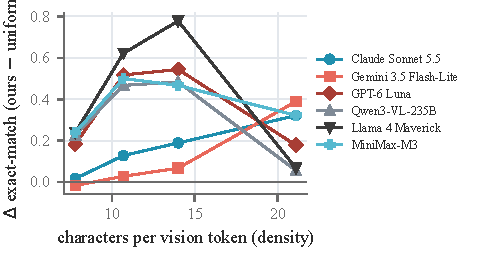
\includegraphics[width=\columnwidth]{fig/phase.pdf}
\caption{Gain in identifier exact-match of reallocation over uniform rendering versus rendering density (short synthetic documents, $N{=}30$ per point).}
\label{fig:phase}
\end{figure}

\paragraph{Readers do not know when they misread.}
Allowing an ``[unreadable]'' answer did not consistently reduce silent errors: MiniMax-M3 used it for at most 6\% of identifiers, and its rate of wrong-but-well-formed answers fell in one of four conditions (uniform, 21 characters per vision token: 0.40 to 0.31) and rose in the other three.
This supports preventing errors at render time rather than relying on the reader's self-assessment.

\paragraph{Agent-based readers can leak across items.}
In a pilot, Claude readers accessed through an agent interface read several images in one session.
Among their wrong prose answers, 50--100\% were names that appeared in \emph{other} images of the same session, versus 0--10\% for MiniMax-M3 queried statelessly.
All agent-based readings reported in this paper therefore use a Latin-square design in which each agent sees each item in only one form (\cref{app:claude}).

\section{Negative Results}
\label{app:negative}

\paragraph{Global detector.}
A detector that also flagged four-digit numbers and long letter-only tokens (later replaced by the one in \cref{sec:detect}) flagged on average 85 and 112 words per MultiFieldQA and HotpotQA document, 62\% of them years.
On one LongBench sample it lowered F1 by 0.05 on average, with 3 of 12 cells significantly negative; on a second sample it was neutral ($-$0.005, 1 of 12 negative).
With the final detector the difference to uniform rendering is $+$0.000 (0 of 12 negative) on the second sample.

\paragraph{Word wrapping.}
Wrapping prose at word boundaries wastes part of every line; on long documents at the 5\,px budget this left no room to enlarge anything, so that variant matched or exceeded the uniform cost while gaining little ($+$0.00 to $+$0.12 recall).
Character wrapping for prose (\cref{sec:allocate}) removes this waste.

\paragraph{Local instead of global shrinking.}
Shrinking only the prose within $K$ words of a flagged string, with the smallest feasible $K$, was harmless on LongBench ($+$0.003, 0 of 12 negative) but retained only 84\% of the RULER gain at the 6\,px budget, because it fills the whole budget with slightly smaller enlarged strings.
It brought no benefit over global shrinking.

\paragraph{Other variants.}
On short manifests, enlarging only the hash and path substrings of a manifest line freed almost no space.
Adding one pixel of line spacing to prose-only lines did not change prose accuracy ($+$0.00, 95\% CI $[-0.09,0.09]$).
Keeping prose at the uniform size left room only for 6--8\,px identifiers and recovered 13--24 points less than full reallocation.

\section{Hazard Density and Routing}
\label{app:density}

\begin{figure*}[t]
\centering
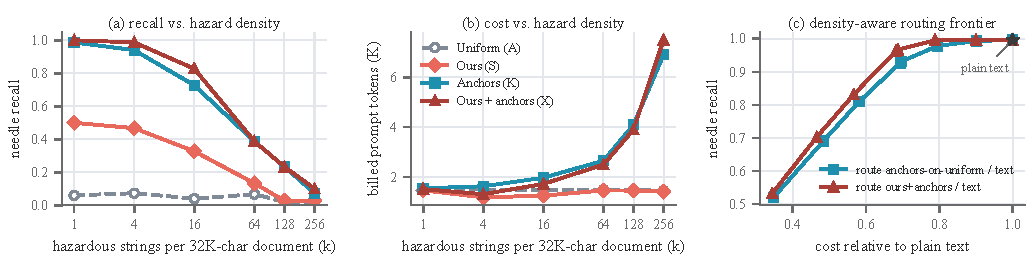
\includegraphics[width=\textwidth]{fig/density.pdf}
\caption{\textbf{Hazard density.} 32K-character documents with $k$ UUID needles, one of which is queried ($N{=}25$). (a) Recall and (b) billed tokens for uniform rendering (A), our allocation (S), anchors on uniform rendering (K), and our allocation with anchors (X); recall averages the five non-Claude readers; cost averages the readers that report usage (Claude included, MiniMax excluded). (c) Recall versus cost relative to plain text when each document is routed either to an image with anchors or to plain text by \cref{eq:route}, sweeping $\tau$ (the four readers with billed costs for both images and plain text).}
\label{fig:density}
\end{figure*}

\Cref{fig:density} varies the number of flagged strings per 32K-character document from 1 to 256 (per-reader values, including Claude, in \cref{tab:app_density}).
Allocation alone degrades as density grows (0.42 at $k{=}1$, 0.24 at $k{=}16$, 0.06 at $k{=}64$), because more strings compete for the pixels prose can give up.
Anchors are strong while hazards are sparse but become both less accurate and expensive as they multiply, reaching 0.34 recall (K) at $k{=}64$ for 1.8$\times$ the tokens of uniform rendering.
At $k{=}4$, X recovers 0.98 of the needles while costing 13\% less than uniform rendering and 20\% less than K.
Under the precision-aware F1, however, X and K do not differ (pooled over $k\in\{1,4,16\}$: $-$0.01, CI [$-$0.07, 0.04]), and several readers return most of the anchor list at $k\ge4$.
For routing, $\tau$ was chosen per reader by two-fold cross-validation on this sweep; the selected values have median 0.3.
Sweeping $\tau$ traces the recall--cost frontiers of panel (c), on which routing with X matches or dominates routing with K; at $\tau{=}0.3$ it reaches 0.97 recall at 0.69$\times$ the plain-text cost versus 0.93 at 0.70$\times$.
These frontiers are computed on the same sweep used to select $\tau$ and should be read as in-sample.

\begin{table}[h]
\centering\small\setlength{\tabcolsep}{3pt}
\caption{Per-reader recall in the hazard-density sweep, K/X (anchors on uniform rendering / on our rendering).}
\label{tab:app_density}
\resizebox{\columnwidth}{!}{%
\begin{tabular}{l cccccc}
\toprule
Reader & $k{=}1$ & 4 & 16 & 64 & 128 & 256 \\
\midrule
Claude Sonnet 5.5 & 1.00/1.00 & 1.00/1.00 & 0.88/0.96 & 0.60/0.72 & 0.28/0.44 & 0.16/0.24 \\
Gemini 3.5 Flash-Lite & 0.96/1.00 & 0.96/1.00 & 0.68/0.88 & 0.36/0.28 & 0.28/0.16 & 0.08/0.08 \\
GPT-6 Luna & 0.96/1.00 & 0.88/1.00 & 0.60/0.92 & 0.32/0.32 & 0.20/0.12 & 0.12/0.12 \\
Qwen3-VL-235B & 1.00/1.00 & 1.00/1.00 & 1.00/1.00 & 0.04/0.04 & 0.00/0.00 & 0.00/0.00 \\
Llama 4 Maverick & 1.00/1.00 & 0.80/0.96 & 0.48/0.44 & 0.48/0.20 & 0.16/0.16 & 0.08/0.04 \\
MiniMax-M3 & 1.00/1.00 & 1.00/0.96 & 0.72/0.76 & 0.52/0.76 & 0.48/0.52 & 0.00/0.12 \\
\bottomrule
\end{tabular}}
\end{table}


\section{Natural-Identifier Questions}
\label{app:niq}

For each of six LongBench tasks we shuffled the documents of at most 40K characters with a fixed seed and kept the first ten that contain a usable target.
A target is a word flagged by the detector of \cref{sec:detect} that, after stripping surrounding punctuation, has 6--64 ASCII characters including a digit, starts with a letter or digit, and is preceded by six words none of which is flagged; the six-word phrase must occur exactly once in the document.
We exclude dataset artifacts: Qasper reference placeholders (e.g., \texttt{BIBREF}), formula fragments, characters replaced by ``?'' during ASCII normalization, and words glued across a missing space (a comma directly followed by a letter, a period or closing parenthesis followed by an uppercase letter, and a few letter--digit patterns); targets containing ``='' are also excluded.
A first version of the set without the last two filters contained such artifacts in 14 of its 60 questions; because anchors and enlarged rendering present the glued string as a single unit, that version favored our arms, and we discarded it.
The prompt asks for the exact string that follows the phrase; scoring is the same recall as for RULER.
The same 60 questions were also rendered at base sizes of 5 and 7\,px for the frontier of \cref{sec:anchors}.

\paragraph{Detector-independent set.}
To measure what happens to strings the detector misses, a second set (new seed) samples the target uniformly from all tokens of 4--64 ASCII characters that contain a digit, with the same phrase and artifact filters (including \texttt{EQREF} and \texttt{DISPLAYFORM} placeholders) but without requiring the detector to flag the target or the document.
The detector flags one of the 60 targets.

\section{Real-Corpus Profile}
\label{app:corpora}

\Cref{tab:app_corpora} lists the routing profile of real corpora: 13 English LongBench tasks (20 chunks each), Paul Graham essays, Python source files from an installed package environment, local system logs, and Python package \texttt{RECORD} manifests (36--40 chunks each).
Every chunk is rendered and reallocated so that $r$ uses the actual image cost.

\begin{table}[!htbp]
\centering\footnotesize\setlength{\tabcolsep}{2.2pt}
\caption{Routing profile of real corpora (32K-character chunks, $\tau{=}0.3$). Flags per 1K characters, median and 90th-percentile routing ratio $r$, share routed to image+anchors (X), and estimated cost relative to plain text. Text tokens are estimated with a linear fit to billed text-only reads (0.208 tokens per ordinary and 0.737 per flagged character; mean absolute relative error 1.1\%).}
\label{tab:app_corpora}
\begin{tabular}{l c c c c c c}
\toprule
Corpus & $n$ & flags/1K & $r$ med & $r$ p90 & $\to$X & cost/T \\
\midrule
LB/narrativeqa & 20 & 0.06 & 0.00 & 0.01 & 95\% & 0.27 \\
LB/qasper & 20 & 0.18 & 0.03 & 0.13 & 100\% & 0.19 \\
LB/multifieldqa\_en & 20 & 0.85 & 0.05 & 0.98 & 75\% & 0.43 \\
LB/hotpotqa & 20 & 0.17 & 0.01 & 0.11 & 95\% & 0.25 \\
LB/2wikimqa & 20 & 0.06 & 0.01 & 0.05 & 100\% & 0.21 \\
LB/musique & 20 & 0.06 & 0.00 & 0.02 & 100\% & 0.22 \\
LB/gov\_report & 20 & 0.04 & 0.00 & 0.02 & 100\% & 0.21 \\
LB/qmsum & 20 & 0.00 & 0.00 & 0.00 & 100\% & 0.23 \\
LB/multi\_news & 20 & 0.06 & 0.00 & 0.05 & 100\% & 0.21 \\
LB/triviaqa & 20 & 0.23 & 0.08 & 0.19 & 95\% & 0.23 \\
LB/passage\_retrieval\_en & 20 & 0.04 & 0.00 & 0.02 & 100\% & 0.21 \\
LB/lcc & 20 & 1.40 & 0.40 & 0.83 & 25\% & 0.81 \\
LB/repobench-p & 20 & 1.43 & 0.52 & 0.87 & 5\% & 0.96 \\
pg\_essays & 36 & 0.01 & 0.00 & 0.00 & 100\% & 0.22 \\
python\_source & 40 & 2.62 & 0.67 & 1.47 & 12\% & 0.91 \\
system\_logs & 40 & 11.84 & 3.73 & 4.09 & 0\% & 1.00 \\
pkg\_manifests & 40 & 11.32 & 16.09 & 16.72 & 0\% & 1.00 \\
\bottomrule
\end{tabular}
\end{table}


\section{Additional Claude Reader}
\label{app:claude}

We also used Claude through an agent interface as a reader that is never used to choose any setting.
For $k\in\{1,4,16,64,256\}$, ten items of the density sweep were read as X, K, and plain text in a Latin square: 15 agents each read ten different items, each in one form, using only a file-reading tool and a tool to write their answer file.
Costs are estimated with \cref{eq:vtok} for images and with the linear text-token fit of \cref{tab:app_corpora}.
\Cref{tab:app_claude} shows that this stronger reader tolerates higher density than the API readers (0.90 for X at $k{=}64$, against 0.60 for K), and with $\tau{=}0.3$ the routed system reaches 0.98 recall at an estimated 0.61$\times$ the plain-text cost.
Agents may resample images when reading them, and $N{=}10$ per cell is small, so these numbers are indicative.

\begin{table}[h]
\centering\small\setlength{\tabcolsep}{4pt}
\caption{Additional Claude reader (agent interface, one item per form per agent; $N{=}10$ per cell). Recall and estimated cost relative to plain text.}
\label{tab:app_claude}
\begin{tabular}{c ccc cc}
\toprule
$k$ & X & K & T & cost X/T & cost K/T \\
\midrule
1 & 1.00 & 1.00 & 1.00 & 0.23 & 0.23 \\
4 & 1.00 & 1.00 & 1.00 & 0.17 & 0.24 \\
16 & 0.90 & 1.00 & 1.00 & 0.22 & 0.27 \\
64 & 0.90 & 0.60 & 1.00 & 0.36 & 0.36 \\
256 & 0.20 & 0.00 & 1.00 & 0.59 & 0.60 \\
\bottomrule
\end{tabular}
\end{table}


\section{Reproducibility and Ethics}
\label{app:repro}

\paragraph{Prior work.}
The detector design, anchors, and text routing follow~\cite{anon2026renderretain}, which is under review; an anonymized copy is included in the supplementary material.

\paragraph{Code and data.}
The renderer, detector, router, task generators, reader clients, analysis scripts, all logged model outputs, and the scripts that produce every figure and table will be released.
Task data are generated from public sources (RULER templates with Paul Graham essays, LongBench) with fixed seeds.

\paragraph{Compute and cost.}
No model was trained.
All readers were accessed through provider APIs between November 1 and 4, 2026; reader versions are identified by their provider model names in \cref{sec:setup}.
Pay-per-token API charges for all experiments, including pilots, were about \$55; MiniMax-M3 and the agent-based Claude reader were used under subscription plans.

\paragraph{Ethics.}
The study involves no human subjects and no personal data.
The system logs profiled in \cref{app:corpora} were processed locally to count flagged strings; their contents are not released.
Better verbatim fidelity under compression could in principle help extract identifiers from rendered documents, but the method only changes how a document the user already holds is presented to a model.
